\documentclass[man]{apa6}
\usepackage{lmodern}
\usepackage{amssymb,amsmath}
\usepackage{ifxetex,ifluatex}
\usepackage{fixltx2e} % provides \textsubscript
\ifnum 0\ifxetex 1\fi\ifluatex 1\fi=0 % if pdftex
  \usepackage[T1]{fontenc}
  \usepackage[utf8]{inputenc}
\else % if luatex or xelatex
  \ifxetex
    \usepackage{mathspec}
  \else
    \usepackage{fontspec}
  \fi
  \defaultfontfeatures{Ligatures=TeX,Scale=MatchLowercase}
\fi
% use upquote if available, for straight quotes in verbatim environments
\IfFileExists{upquote.sty}{\usepackage{upquote}}{}
% use microtype if available
\IfFileExists{microtype.sty}{%
\usepackage{microtype}
\UseMicrotypeSet[protrusion]{basicmath} % disable protrusion for tt fonts
}{}
\usepackage{hyperref}
\hypersetup{unicode=true,
            pdftitle={Measures and Descriptive Statistics},
            pdfauthor={Karen Santamaria, Yifan Ma, Caroline Li, \& Jane Bang},
            pdfborder={0 0 0},
            breaklinks=true}
\urlstyle{same}  % don't use monospace font for urls
\usepackage{graphicx,grffile}
\makeatletter
\def\maxwidth{\ifdim\Gin@nat@width>\linewidth\linewidth\else\Gin@nat@width\fi}
\def\maxheight{\ifdim\Gin@nat@height>\textheight\textheight\else\Gin@nat@height\fi}
\makeatother
% Scale images if necessary, so that they will not overflow the page
% margins by default, and it is still possible to overwrite the defaults
% using explicit options in \includegraphics[width, height, ...]{}
\setkeys{Gin}{width=\maxwidth,height=\maxheight,keepaspectratio}
\IfFileExists{parskip.sty}{%
\usepackage{parskip}
}{% else
\setlength{\parindent}{0pt}
\setlength{\parskip}{6pt plus 2pt minus 1pt}
}
\setlength{\emergencystretch}{3em}  % prevent overfull lines
\providecommand{\tightlist}{%
  \setlength{\itemsep}{0pt}\setlength{\parskip}{0pt}}
\setcounter{secnumdepth}{0}
% Redefines (sub)paragraphs to behave more like sections
\ifx\paragraph\undefined\else
\let\oldparagraph\paragraph
\renewcommand{\paragraph}[1]{\oldparagraph{#1}\mbox{}}
\fi
\ifx\subparagraph\undefined\else
\let\oldsubparagraph\subparagraph
\renewcommand{\subparagraph}[1]{\oldsubparagraph{#1}\mbox{}}
\fi

%%% Use protect on footnotes to avoid problems with footnotes in titles
\let\rmarkdownfootnote\footnote%
\def\footnote{\protect\rmarkdownfootnote}


  \title{Measures and Descriptive Statistics}
    \author{Karen Santamaria\textsuperscript{1}, Yifan Ma\textsuperscript{1}, Caroline Li\textsuperscript{1}, \& Jane Bang\textsuperscript{1}}
    \date{}
  
\shorttitle{SDS/PSY 365}
\affiliation{
\vspace{0.5cm}
\textsuperscript{1} Smith College}
\usepackage{csquotes}
\usepackage{upgreek}
\captionsetup{font=singlespacing,justification=justified}

\usepackage{longtable}
\usepackage{lscape}
\usepackage{multirow}
\usepackage{tabularx}
\usepackage[flushleft]{threeparttable}
\usepackage{threeparttablex}

\newenvironment{lltable}{\begin{landscape}\begin{center}\begin{ThreePartTable}}{\end{ThreePartTable}\end{center}\end{landscape}}

\makeatletter
\newcommand\LastLTentrywidth{1em}
\newlength\longtablewidth
\setlength{\longtablewidth}{1in}
\newcommand{\getlongtablewidth}{\begingroup \ifcsname LT@\roman{LT@tables}\endcsname \global\longtablewidth=0pt \renewcommand{\LT@entry}[2]{\global\advance\longtablewidth by ##2\relax\gdef\LastLTentrywidth{##2}}\@nameuse{LT@\roman{LT@tables}} \fi \endgroup}


\DeclareDelayedFloatFlavor{ThreePartTable}{table}
\DeclareDelayedFloatFlavor{lltable}{table}
\DeclareDelayedFloatFlavor*{longtable}{table}
\makeatletter
\renewcommand{\efloat@iwrite}[1]{\immediate\expandafter\protected@write\csname efloat@post#1\endcsname{}}
\makeatother

\authornote{

Correspondence concerning this article should be addressed to Karen Santamaria, 1 Chapin Way, Unit 7766, Northampton, MA 01063. E-mail: \href{mailto:sanmakaren@gmail.com}{\nolinkurl{sanmakaren@gmail.com}}}



\begin{document}
\maketitle

\hypertarget{method}{%
\section{Method}\label{method}}

\hypertarget{participant-recruitment}{%
\subsection{Participant Recruitment}\label{participant-recruitment}}

The data come from a larger longitudinal study on the transition to parenthood. To be included, couples had to be first time parents and adopting their first child. Adoption agencies across the US were asked to provide study information to clients seeking to adopt. Effort was made to contact agencies in states that had a high percentage of same-sex couples. Over 30 agencies provided information to clients; interested clients contacted the principal investigator for participation details. Both same-sex and heterosexual couples were targeted through these agencies to facilitate similarity on income and geographic location. Organizations such as the Human Rights Campaign, a gay political organization, also disseminated study information.

\hypertarget{procedure}{%
\subsection{Procedure}\label{procedure}}

Both members of each couple were informed of the risks and benefits of the study, gave consent, and participated at pre-adoptive placement (Time 1 or T1) and 2 years post-adoptive placement (T2). At each phase, they were sent a packet of questionnaires to complete and they were interviewed over the phone. Interviews lasted 1-1.5 hours.

\hypertarget{measures}{%
\subsection{Measures}\label{measures}}

\textbf{Parents Relationship.}
Parents' relationship was assessed using the Relationship Questionnaire by Braiker and Kelley(Goldberg, Smith, and Kashy (2010)). The questionnaire contains four subscales: Love (10 items), Conflict (five items), Ambivalence (five items), and Maintenance (five items). Some example items include \enquote{To what extent do you have a sense of \enquote{belonging with your partner?}} (Love), \enquote{How ambivalent are you about continuing in the relationship with your partner?} (Ambivalence), and \enquote{How often do you and your partner argue?} (Conflict). The questions are answered on a 9-point scale (1 not at all to 9 very much). The scale is reliable, 0.8 for the Love subscale, 0.69 for the Conflict subscale after we dropped one variable (w11mar15\_A), 0.73 for the Ambivalent subscale, and 0.53 for the Maintenance subscale. The intraclass correlation (ICC) were 0.42 (Love), 0.52 (Conflict), 0.23 (Ambivalent), and 0.33 (Maintenance).

\textbf{Attachment}
The Maternal Postnatal Attachment Scale (MPAS; Condon and Corkindale (1997)) is a 19 items self-report questionnaire to assess mother-to-infant attachment. Items are rated on a 2, 3, 4, 5 point rating scale, depending on the item. The questionnaire consists of three subscales: Quality of Attachment (9 items), Absence of Hostility (5 items), and Pleasure in Interaction (5 items). Example items include, \enquote{When I am with the baby I feel tense and anxious,} and \enquote{When I am caring for the baby, I get feelings of annoyance or irritation.} The scale was reliable, alpha = 0.76 The intraclass correlation (ICC) was, ICC = 0.24.

\textbf{Depression}
Depression was assessed using the Center for Epidemiological Studies-Depression Scale (CES-D), which is a 20-item measure developed by the National Institute of Mental Health by Radloff(Ghunney (2011)). The example questions include \enquote{My sleep was restless} and \enquote{I did not feel like eating; my appetite was poor} on a four-point scale from 0--rarely or none of the time (less than 1 day) to 3-- most or all of the time (5-7 days). The scale was reliable, Cronbach's alpha = 0.88. The intraclass correlation (ICC) was 0.19.

\textbf{Anxiety.}
The Spielberger State-Trait Anxiety Inventory (STAI; Spielberger (1983)) is a 40 items instrument to measure trait anxiety and state anxiety. Due to the purpose of our study, only the Trait Anxiety subscale (20 items) is used to assess anxiety as a personality characteristic using a Likert scale ranging between 1 (not at all) to 4 (very much). Example items include: \enquote{I worry too much over something that really doesn't matter} and \enquote{I am content; I am a steady person.} The scale was reliable, alpha = 0.9. The intraclass correlation (ICC) was, ICC = -0.0058

\hypertarget{results}{%
\section{Results}\label{results}}

\hypertarget{preliminary-analyses}{%
\subsection{Preliminary Analyses}\label{preliminary-analyses}}

There are 282 individuals recorded in the study where an Actor and a Partner are both present. Within the scope of this study we will exclusively working with these 282 individuals, 141 dyads.
The dyad relationships were 39.0\% heterosexual, 33.3\% lesbian, and 27.7\% gay.
The gender makeup of the study is, 52.8\% female and 47.2\% male.
There are 31 racial/ethnic groups identified in the study with the 8 largest groups being: Caucasian (31.9\%), African American (9.93\%), 1/2 African American and 1/2 Caucasian (7.80\%), Hispanic (7.80\%), Guatemalan (7.45\%), Chinese (7.09\%),Vietnamese (3.55\%), 1/2 Caucasion and 1/2 Hispanic (3.19\%).
The median personal income for participants in the study was \$55,00 during phase 11 and \$60,000 during phase 14.
The median age when a child came to be with their parent was 0 years however something to note is that there is one instance where the recorded age was 72, which may due to error in the data.
The main reason for adoption in this study was due to infertility (43.3\%).
The dyads were categorized as POC-POC (66.0\%), white-white (32.6\%), POC-white(0.709), and NA-NA (0.709). White was loosly defined as those that idenitified as Caucasian, Mostly Caucasian (1/8 American Indian), and Mostly White and POC was an used for all others that were not categorized as white.
In terms of education, 32.3\% of individuals in this study have a Master's, 30.9\% have completed college, 14.2\% did not repoort education level, 9.57\% had a PhD, JD or MD, 6.03\% had some college, 3.90\% had a high school diploma, and 3.19\% had an Associate's.

By using an ANOVA test we found that sexual orientation (homosexual or heterosexual) was a statistically significant predictor for relationship duration at phase 11. On average, homosexual couples in this study have been in a relationship for 1.7557 years less than heterosexual couples.

\begin{verbatim}
## Warning: Removed 15 rows containing non-finite values (stat_boxplot).
\end{verbatim}

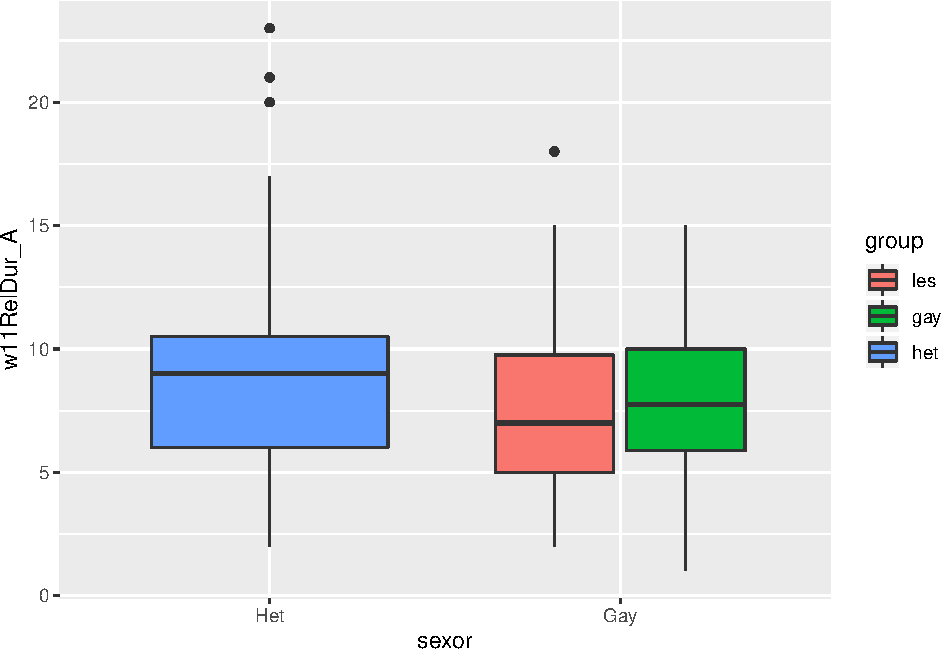
\includegraphics{measures_descriptive_stats_files/figure-latex/unnamed-chunk-3-1.pdf}

\newpage

\hypertarget{references}{%
\section{References}\label{references}}

\begingroup
\setlength{\parindent}{-0.5in}
\setlength{\leftskip}{0.5in}

\hypertarget{refs}{}
\leavevmode\hypertarget{ref-condon1997correlates}{}%
Condon, J. T., \& Corkindale, C. (1997). The correlates of antenatal attachment in pregnant women. \emph{British Journal of Medical Psychology}, \emph{70}(4), 359--372.

\leavevmode\hypertarget{ref-ghunney2011beyond}{}%
Ghunney, A. K.-K. (2011). Beyond race and ethnicity: Predictors of maternal depressive symptoms across the transition to parenthood.

\leavevmode\hypertarget{ref-goldberg2010preadoptive}{}%
Goldberg, A. E., Smith, J. Z., \& Kashy, D. A. (2010). Preadoptive factors predicting lesbian, gay, and heterosexual couples' relationship quality across the transition to adoptive parenthood. \emph{Journal of Family Psychology}, \emph{24}(3), 221.

\leavevmode\hypertarget{ref-spielberger1983state}{}%
Spielberger, C. D. (1983). State-trait anxiety inventory for adults.

\endgroup


\end{document}
